% !TEX TS-program = pdflatex
% !TEX encoding = UTF-8 Unicode

% This is a simple template for a LaTeX document using the "article" class.
% See "book", "report", "letter" for other types of document.

\documentclass[11pt]{article} % use larger type; default would be 10pt

\usepackage[utf8]{inputenc} % set input encoding (not needed with XeLaTeX)
\usepackage{alltt}
\usepackage{graphicx}
\usepackage{amsmath}
\newcommand*\diff{\mathop{}\!\mathrm{d}}

%%% Examples of Article customizations
% These packages are optional, depending whether you want the features they provide.
% See the LaTeX Companion or other references for full information.

%%% PAGE DIMENSIONS
\usepackage{geometry} % to change the page dimensions
\geometry{a4paper} % or letterpaper (US) or a5paper or....
% \geometry{margin=2in} % for example, change the margins to 2 inches all round
% \geometry{landscape} % set up the page for landscape
%   read geometry.pdf for detailed page layout information

\usepackage{graphicx} % support the \includegraphics command and options

% \usepackage[parfill]{parskip} % Activate to begin paragraphs with an empty line rather than an indent

%%% PACKAGES
\usepackage{booktabs} % for much better looking tables
\usepackage{array} % for better arrays (eg matrices) in maths
\usepackage{paralist} % very flexible & customisable lists (eg. enumerate/itemize, etc.)
\usepackage{verbatim} % adds environment for commenting out blocks of text & for better verbatim
\usepackage{subfig} % make it possible to include more than one captioned figure/table in a single float
\usepackage{amsmath}
% These packages are all incorporated in the memoir class to one degree or another...

%%% HEADERS & FOOTERS
\usepackage{fancyhdr} % This should be set AFTER setting up the page geometry
\pagestyle{fancy} % options: empty , plain , fancy
\renewcommand{\headrulewidth}{0pt} % customise the layout...
\lhead{}\chead{}\rhead{}
\lfoot{}\cfoot{\thepage}\rfoot{}

%%% SECTION TITLE APPEARANCE
\usepackage{sectsty}
\allsectionsfont{\sffamily\mdseries\upshape} % (See the fntguide.pdf for font help)
% (This matches ConTeXt defaults)

%%% ToC (table of contents) APPEARANCE
\usepackage[nottoc,notlof,notlot]{tocbibind} % Put the bibliography in the ToC
\usepackage[titles,subfigure]{tocloft} % Alter the style of the Table of Contents
\renewcommand{\cftsecfont}{\rmfamily\mdseries\upshape}
\renewcommand{\cftsecpagefont}{\rmfamily\mdseries\upshape} % No bold!



\title{Numerical Analysis Homework 2}
\author{Margaret Dorsey}
%\date{} % Activate to display a given date or no date (if empty),
         % otherwise the current date is printed 

\begin{document}
\maketitle

\section*{Problem 1}
No, a degree 3 polynomial cannot intersect a degree 4 polynomial in exactly 5 points - let $f(x)$ be a degree $3$ polynomial, and $g(x)$ be degree 4. Any intersection of $f$ and $g$
must be a root of $f-g$ and $g-f$, which are degree 4 polynomials, and therefore may have at most $4$ real roots. 

\par It is, however, possible for $f$ and $g$ to intersect at exactly four points. Consider $f(x) = x^3$, and $g(x) = x^4 + 3x^3 - 12x^2 - 2x + 6$. Their difference,
$x^4+2x^3-12x^2 - 2x +6$, is plotted below and clearly has exactly $4$ distinct real roots. $f$ and $g$ can intersect only at those roots, and must intersect at them, so thus $f$ and $g$ intersect
exactly 4 times, as shown on the second plot. 

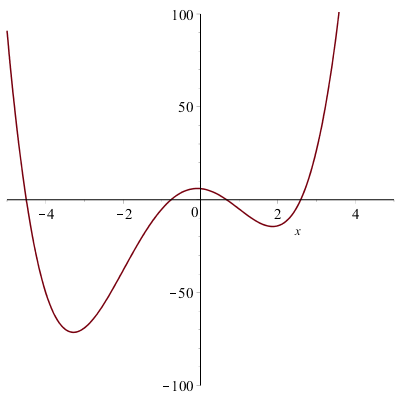
\includegraphics[width=0.5\textwidth]{plots/problem1plot1.png}
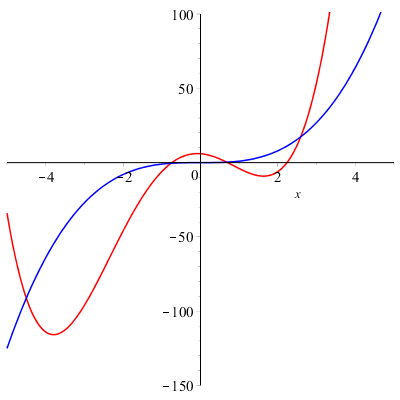
\includegraphics[width=0.5\textwidth]{plots/problem1plot2.png}
\section*{Problem 2}
Using the formula $$P_n(x) - \sum_{j=1}^n y_j \prod_{k=1, k \neq j}^n \frac{x-x_k}{x_j - x_k}$$
we obtain
	$$P_2(x) = \frac{(x-2)(x-4)}{3}\cdot 0 + \frac{(x-1)(x-4)}{-2}\cdot \ln2 + \frac{(x-1)(x-2)}{6} \cdot \ln4 $$
	$$P_2(x) =  \frac{-(x-1)(x-4)}{2}\cdot \ln2 + \frac{(x-1)(x-2)}{3} \cdot \ln2 $$
	$$P_2(x) =  \frac{-\ln2}{6}x^2 + \frac{3\ln2}{2}x -  \frac{4\ln2}{3} $$
The graph of this polynomial fit is shown below.
\begin{center}
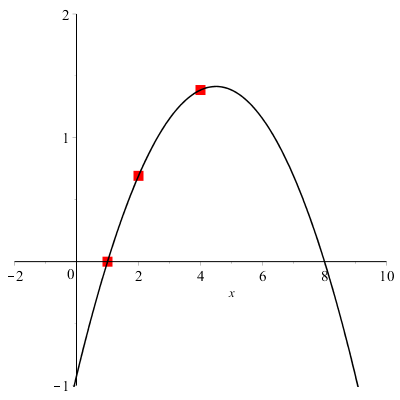
\includegraphics[scale=.5]{plots/problem2plot1.png}
\end{center}
\par Using this approximation, we obtain $\ln 3 \approx P_2(3) =  \frac{-9\ln2}{6} + \frac{9\ln2}{2} -  \frac{4\ln2}{3} = \frac{5}{3} \ln 2 \approx 1.1552453$.
Using the formula
	$$|f(x) - P(x)|\leq \max_{[2,4]}\left| \frac{f^{(n+1)}( \xi)}{(n+1)!} \right| \cdot  \max_{[2,4]} \left| \prod_{i=0}^n(x-x_i) \right|$$
with $f(x) = \ln x$, $f^{(3)}(x) = \frac{2}{x^3}$, we obtain
	$$|f(x) - P(x)|\leq \max_{[2,4]}\left| \frac{1}{3 (\xi)^3} \right| \cdot \max_{[2,4]}  \left| x^3 - 7x^2 + 14x - 8 \right|$$
\par Because $f^{(3)}(\xi)$ is strictly decreasing and non-negative on our interval, we know the maximum on $[2,4]$ is $\frac{1}{24}$ at $2$. Using the derivative of $ x^3 - 7x^2 + 14x - 8$
with the quadratic formula, we find that the maximum absolute value on $[2,4]$ is $-\frac{2}{27}(10 + 7\sqrt7)$ at $x = \frac{7}{3}+\frac{\sqrt7}{3}$, or approximately $2.11261$.
\par Multiplying these values, we obtain $|f(x) - P(x)| \leq .0880255$. \\
\par Comparing our value of  $1.1552453$ to the actual value of $\ln 3 \approx 1.0986123$, we have $|f(x) - P_2(x)| = .056630 < .0880255$, as expected.
\par
\section*{Problem 3}
Using the formulas $B(0) = P_0$ and $B(1) = P_3$, we obtain $P_0 = (1,1)$ and $P_3 = (9,1)$. We then calculate $B'(t) = (x'(t),y'(t)) = (12t+6t^2,3t^2 - 1)$, and note that because in general $B'(t) = 3(1-t)^2(P_1 - P_0) + 6(1-t)t(P_2-P_1) + 3t^2(P_3 - P_2)$, $B'(0) = 3(P_1 - P_0)$ and $B'(1) = 3(P_3 - P_2)$. Thus we have $P_1 = (1,\frac{2}{3})$ and $P_2 = (3,\frac{1}{3})$. This gives us the complete set of control points for the curve, namely
$$\{(1,1),  (1,\frac{2}{3}),   (3,\frac{1}{3}), (9,1) \}$$
\section*{Problem 4}

We first note that 
$$\begin{array}{lclcl} A_1 & = &  \frac{x_2 - x}{x_2 - x_1} & = & 1-x \\
		        A_2 & = & \frac{x_3 - x}{x_3 - x_2} & = & 2-x \\
		        A_3 & = & \frac{x_4 - x}{x_4 - x_3} & = & 3-x 
\end{array}$$

$$\begin{array}{lclcl} B_1 & = &  \frac{x - x_1}{x_2 - x_1} & = & x - 0 \\
		        B_2 & = & \frac{x -x_2}{x_3 - x_2} & = & x - 1 \\
		        B_3 & = & \frac{x - x_3}{x_4 - x_3} & = & x - 2 
\end{array}$$

$$\begin{array}{lclcl} C_1 & = &  \frac{(x_2 - x_1)^2}{6}[A_1^3 - A_1] & = & \frac{1}{6}(-x^3 + 3x^2 - 2x) \\
		        C_2 & =&  \frac{(x_3 - x_2)^2}{6}[A_2^3 - A_2] & = &\frac{1}{6}(-x^3 + 6x^2 - 11x + 6) \\
		        C_3 & =&  \frac{(x_4 - x_3)^2}{6}[A_3^3 - A_3] & = & \frac{1}{6}(-x^3 + 9x^2 - 26x + 24) 
\end{array}$$

$$\begin{array}{lclcl} D_1 & = &  \frac{(x_2 - x_1)^2}{6}[B_1^3 - B_1] & = & \frac{1}{6}(x^3 - x) \\
		        D_2 & =&  \frac{(x_3 - x_2)^2}{6}[B_2^3 - B_2] & = &\frac{1}{6}(x^3 - 3x^2 + 2x) \\
		        D_3 & =&  \frac{(x_4 - x_3)^2}{6}[B_3^3 - B_3] & = & \frac{1}{6}(x^3 - 6x^2 + 11x - 6) 
\end{array}$$

%%%%%%%%%%%%%%%%%%%%%%%%%%%%%%%%%%%%%%%%%%%%%%%%%%%
\subsection*{Natural Endpoint Condition} 
$$\begin{bmatrix} 1 & 0 & 0 & 0 \\ x_2 - x_1 & 2(x_3 - x_1) & x_3 - x_2 & 0 
		 \\ 0 & x_3 - x_2 & 2(x_4 - x_2) & x_4 - x_3 \\ 0 & 0 & 0 & 1
\end{bmatrix}
\begin{bmatrix} y_1'' \\ y_2'' \\ y_3'' \\ y_4'' \end{bmatrix} = 
\begin{bmatrix} 0 \\ 6\left( \frac{y_3 - y_2}{x_3 - x_2} - \frac{y_2-y_1}{x_2 - x_1} \right) \\ 
			 6\left( \frac{y_4 - y_3}{x_4 - x_3} - \frac{y_3-y_2}{x_3 - x_2} \right) \\ 0\end{bmatrix}$$

$$\begin{bmatrix} 1 & 0 & 0 & 0 \\ 1 - 0 & 2(2 -0) &2 -1 & 0 
		 \\ 0 & 2 - 1 & 2(3 -1) & 3 - 2 \\ 0 & 0 & 0 & 1
\end{bmatrix}
\begin{bmatrix} y_1'' \\ y_2'' \\ y_3'' \\ y_4'' \end{bmatrix} = 
\begin{bmatrix} 0 \\  6\left( \frac{2 - 5}{2 - 1} - \frac{5-3}{1 - 0} \right) \\ 
			 6\left( \frac{1 - 2}{3 - 2} - \frac{2-5}{2 - 1} \right) \\ 0\end{bmatrix}$$

$$\begin{bmatrix} 1 & 0 & 0 & 0 \\ 1 & 4 &1 & 0 
		 \\ 0 & 1 & 4 & 1 \\ 0 & 0 & 0 & 1
\end{bmatrix}
\begin{bmatrix} y_1'' \\ y_2'' \\ y_3'' \\ y_4'' \end{bmatrix} = 
\begin{bmatrix} 0 \\ -30 \\ 12 \\ 0\end{bmatrix}$$

$$
\begin{bmatrix} y_1'' \\ y_2'' \\ y_3'' \\ y_4'' \end{bmatrix} = 
\begin{bmatrix} 1 & 0 & 0 & 0 \\ -\frac{4}{15} & \frac{4}{15} & -\frac{1}{15} & \frac{1}{15} 
		 \\  \frac{1}{15} & -\frac{1}{15} & \frac{4}{15} & -\frac{4}{15} \\ 0 & 0 &0 & 1
\end{bmatrix}
\begin{bmatrix} 0 \\ -30 \\ 12 \\ 0\end{bmatrix}$$

$$
\begin{bmatrix} y_1'' \\ y_2'' \\ y_3'' \\ y_4'' \end{bmatrix} = 
\begin{bmatrix} 0 \\ -\frac{44}{5} \\\frac{26}{5} \\ 0\end{bmatrix}$$

Using these derived values of $y_i''$ with our $A$,$B$,$C$, and $D$ equations above, we have

$$\begin{array}{lclcl} y^{(cubic)}_1 & = &  y_1A_1 + y_2B_1 + y_1''C_1 + y_2'' D_1 & = 
							& -\frac{22}{15}x^3 + \frac{52}{15}x + 3\\
		        y^{(cubic)}_2  & = & y_2A_2 + y_3B_2 + y_2''C_2 + y_3'' D_2 & = 
							&  \frac{7}{3}x^3 - \frac{57}{5}x^2 + \frac{223}{15}x - \frac{4}{5}\\
		        y^{(cubic)}_3  & = & y_3A_3 + y_4B_3 + y_3''C_3 + y_4'' D_3 & =
							& -\frac{13}{15}x^3 + \frac{39}{5}x^2 - \frac{353}{15}x + \frac{124}{5}
\end{array}$$

\begin{center}
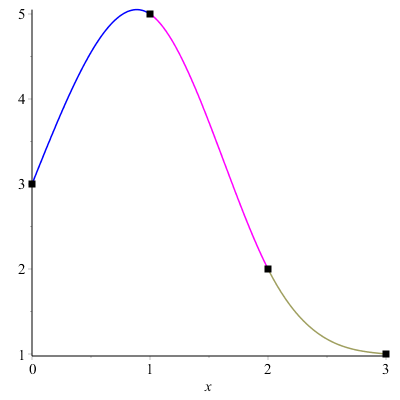
\includegraphics[scale=.5]{plots/problem4plot1.png}
\end{center}
%%%%%%%%%%%%%%%%%%%%%%%%%%%%%%%%%%%%%%%%%%%%%%%%%%%%
\subsection*{Curvature-Adjusted Endpoint Condition}
$$\begin{bmatrix} 1 & 0 & 0 & 0 \\ x_2 - x_1 & 2(x_3 - x_1) & x_3 - x_2 & 0 
		 \\ 0 & x_3 - x_2 & 2(x_4 - x_2) & x_4 - x_3 \\ 0 & 0 & 0 & 1
\end{bmatrix}
\begin{bmatrix} y_1'' \\ y_2'' \\ y_3'' \\ y_4'' \end{bmatrix} = 
\begin{bmatrix} k_1 \\ 6\left( \frac{y_3 - y_2}{x_3 - x_2} - \frac{y_2-y_1}{x_2 - x_1} \right) \\ 
			 6\left( \frac{y_4 - y_3}{x_4 - x_3} - \frac{y_3-y_2}{x_3 - x_2} \right) \\ k_n\end{bmatrix}$$

$$\begin{bmatrix} 1 & 0 & 0 & 0 \\ 1 - 0 & 2(2 -0) &2 -1 & 0 
		 \\ 0 & 2 - 1 & 2(3 -1) & 3 - 2 \\ 0 & 0 & 0 & 1
\end{bmatrix}
\begin{bmatrix} y_1'' \\ y_2'' \\ y_3'' \\ y_4'' \end{bmatrix} = 
\begin{bmatrix} k_n \\  6\left( \frac{2 - 5}{2 - 1} - \frac{5-3}{1 - 0} \right) \\ 
			 6\left( \frac{1 - 2}{3 - 2} - \frac{2-5}{2 - 1} \right) \\ k_n\end{bmatrix}$$

$$\begin{bmatrix} 1 & 0 & 0 & 0 \\ 1 & 4 &1 & 0 
		 \\ 0 & 1 & 4 & 1 \\ 0 & 0 & 0 & 1
\end{bmatrix}
\begin{bmatrix} y_1'' \\ y_2'' \\ y_3'' \\ y_4'' \end{bmatrix} = 
\begin{bmatrix} k_1 \\ -30 \\ 12 \\ k_n\end{bmatrix}$$

Choosing $k_1 = 100$, $k_2 = -100$, we have 

$$
\begin{bmatrix} y_1'' \\ y_2'' \\ y_3'' \\ y_4'' \end{bmatrix} = 
\begin{bmatrix} 1 & 0 & 0 & 0 \\ -\frac{4}{15} & \frac{4}{15} & -\frac{1}{15} & \frac{1}{15} 
		 \\  \frac{1}{15} & -\frac{1}{15} & \frac{4}{15} & -\frac{4}{15} \\ 0 & 0 &0 & 1
\end{bmatrix}
\begin{bmatrix} 100 \\ -30 \\ 12 \\ -100\end{bmatrix}$$

$$
\begin{bmatrix} y_1'' \\ y_2'' \\ y_3'' \\ y_4'' \end{bmatrix} = 
\begin{bmatrix} 100 \\ -\frac{632}{15} \\\frac{578}{15} \\ -100\end{bmatrix}$$

$$\begin{array}{lclcl} y^{(cubic)}_1 & = & -\frac{1066}{45} + 50x^2 - \frac{1094}{45}x + 3  \\
		        y^{(cubic)}_2  & = & \frac{121}{9}x^3 - \frac{307}{5}x^2 + \frac{3919}{45}x - \frac{512}{15} \\
		        y^{(cubic)}_3  & = & -\frac{1039}{45} + \frac{789}{5}x^2 - \frac{15809}{45}x + \frac{3872}{15}
\end{array}$$

\begin{center}
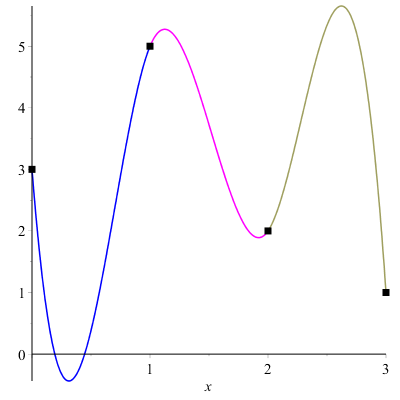
\includegraphics[scale=.5]{plots/problem4plot2.png}
\end{center}
%%%%%%%%%%%%%%%%%%%%%%%%%%%%%%%%%%%%%%%%%%%%%%%%%%%%

\subsection*{Clamped Endpoint Condition}
$$\begin{bmatrix} 2 & 1 & 0 & 0 \\ x_2 - x_1 & 2(x_3 - x_1) & x_3 - x_2 & 0 
		 \\ 0 & x_3 - x_2 & 2(x_4 - x_2) & x_4 - x_3 \\ 0 & 0 & 1 & 2
\end{bmatrix}
\begin{bmatrix} y_1'' \\ y_2'' \\ y_3'' \\ y_4'' \end{bmatrix} = 
\begin{bmatrix} 6\left(  \frac{y_2-y_1}{x_2 - x_1} -c_n  \right)\\ 6\left( \frac{y_3 - y_2}{x_3 - x_2} - \frac{y_2-y_1}{x_2 - x_1} \right) \\ 
			 6\left( \frac{y_4 - y_3}{x_4 - x_3} - \frac{y_3-y_2}{x_3 - x_2} \right) \\  6\left( c_n - \frac{y_4 - y_3}{x_4 - x_3} \right)\end{bmatrix}$$

$$\begin{bmatrix} 2 & 1 & 0 & 0 \\ 1 - 0 & 2(2 -0) &2 -1 & 0 
		 \\ 0 & 2 - 1 & 2(3 -1) & 3 - 2 \\ 0 & 0 & 1 & 2
\end{bmatrix}
\begin{bmatrix} y_1'' \\ y_2'' \\ y_3'' \\ y_4'' \end{bmatrix} = 
\begin{bmatrix} 6\left(  \frac{5-3}{1-0} -c_n  \right)\\  6\left( \frac{2 - 5}{2 - 1} - \frac{5-3}{1 - 0} \right) \\ 
			 6\left( \frac{1 - 2}{3 - 2} - \frac{2-5}{2 - 1} \right) \\  6\left( c_n -  \frac{1 - 2}{3 - 2} \right)\end{bmatrix}$$

$$\begin{bmatrix} 2 & 1 & 0 & 0 \\ 1 & 4 &1 & 0 
		 \\ 0 & 1 & 4 & 1 \\ 0 & 0 & 1 & 2
\end{bmatrix}
\begin{bmatrix} y_1'' \\ y_2'' \\ y_3'' \\ y_4'' \end{bmatrix} = 
\begin{bmatrix} 12-6c_n \\ -30 \\ 12 \\ 6(c_n +1) \end{bmatrix}$$

Choosing $c_n = 4$, we have

$$
\begin{bmatrix} y_1'' \\ y_2'' \\ y_3'' \\ y_4'' \end{bmatrix} = 
\frac{1}{45}\begin{bmatrix}26 & -7 & 2 & -1 \\ -7 & 14 & -4 & 2 
		 \\  2 & -4 & 14 & -7 \\ -1 & 2 & -7 & 26
\end{bmatrix}
\begin{bmatrix} -12 \\ -30 \\ 12 \\ 30\end{bmatrix}$$

$$
\begin{bmatrix} y_1'' \\ y_2'' \\ y_3'' \\ y_4'' \end{bmatrix} = 
\begin{bmatrix} -\frac{12}{5} \\ -\frac{36}{5} \\\frac{6}{5} \\ \frac{72}{5}\end{bmatrix}$$

$$\begin{array}{lclcl} y^{(cubic)}_1 & = & -\frac{4}{5}x^3 - \frac{6}{5}x^2 + 4x + 3  \\
		        y^{(cubic)}_2  & = & \frac{7}{5}x^3 - \frac{39}{5}x^2 + \frac{53}{5}x + \frac{4}{5} \\
		        y^{(cubic)}_3  & = & -\frac{11}{5}x^3 - \frac{63}{5}x^2 + \frac{101}{5}x - \frac{28}{5} 
\end{array}$$

\begin{center}
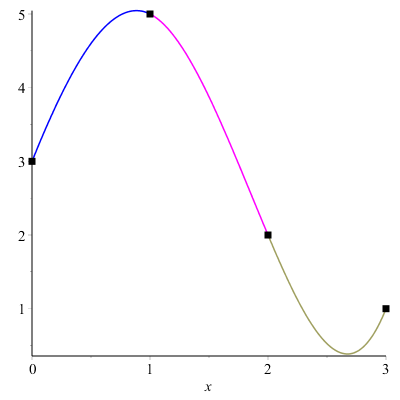
\includegraphics[scale=.5]{plots/problem4plot3.png}
\end{center}

%%%%%%%%%%%%%%%%%%%%%%%%%%%%%%%%%%%%%%%%%%%%%%%%%%%%


\subsection*{Parabolically Terminated Endpoint Condition}

$$\begin{bmatrix} 1 & -1 & 0 & 0 \\ x_2 - x_1 & 2(x_3 - x_1) & x_3 - x_2 & 0 
		 \\ 0 & x_3 - x_2 & 2(x_4 - x_2) & x_4 - x_3 \\ 0 & 0 & -1 & 1
\end{bmatrix}
\begin{bmatrix} y_1'' \\ y_2'' \\ y_3'' \\ y_4'' \end{bmatrix} = 
\begin{bmatrix} 0 \\ 6\left( \frac{y_3 - y_2}{x_3 - x_2} - \frac{y_2-y_1}{x_2 - x_1} \right) \\ 
			 6\left( \frac{y_4 - y_3}{x_4 - x_3} - \frac{y_3-y_2}{x_3 - x_2} \right) \\ 0\end{bmatrix}$$


$$\begin{bmatrix} 1 & -1 & 0 & 0 \\ 1 & 4 &1 & 0 
		 \\ 0 & 1 & 4 & 1 \\ 0 & 0 & -1 & 1
\end{bmatrix}
\begin{bmatrix} y_1'' \\ y_2'' \\ y_3'' \\ y_4'' \end{bmatrix} = 
\begin{bmatrix} 0 \\ -30 \\ 12 \\ 0\end{bmatrix}$$

$$
\begin{bmatrix} y_1'' \\ y_2'' \\ y_3'' \\ y_4'' \end{bmatrix} = 
\frac{1}{24}\begin{bmatrix}19 & 5 & -1 & 1 \\ -5 & 5 & -1 & 1 
		 \\  1 & -1 & 5 & -5 \\ 1 & -1 & 5 & 19
\end{bmatrix}
\begin{bmatrix} 0 \\ -30 \\ 12 \\ 0\end{bmatrix}$$

$$
\begin{bmatrix} y_1'' \\ y_2'' \\ y_3'' \\ y_4'' \end{bmatrix} = 
\begin{bmatrix} -\frac{27}{4} \\ -\frac{27}{4} \\\frac{15}{4} \\ \frac{15}{4}\end{bmatrix}$$

$$\begin{array}{lclcl} y^{(cubic)}_1 & = &  - \frac{27}{8}x^2 + \frac{43}{8} x + 3  \\
		        y^{(cubic)}_2  & = & \frac{13}{8}x^3 - \frac{63}{8}x^2 + \frac{37}{4}x + 2 \\
		        y^{(cubic)}_3  & = & \frac{15}{8}x^2 - \frac{83}{8}x - \frac{61}{4} 
\end{array}$$

\begin{center}
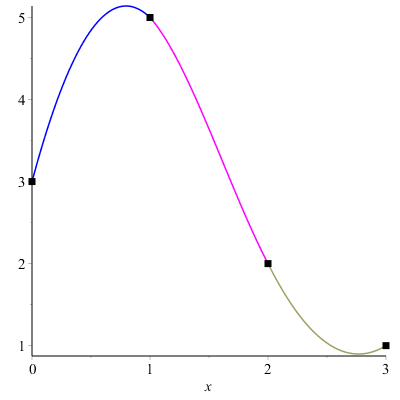
\includegraphics[scale=.5]{plots/problem4plot4.png}
\end{center}



%%%%%%%%%%%%%%%%%%%%%%%%%%%%%%%%%%%%%%%%%%%%%%%%%%%%


\subsection*{Not-a-Knot Endpoint Condition}

$$\begin{bmatrix} x_3 - x_2 & -(x_3- x_1) & x_2 - x_1 & 0 \\ x_2 - x_1 & 2(x_3 - x_1) & x_3 - x_2 & 0 
		 \\ 0 & x_3 - x_2 & 2(x_4 - x_2) & x_4 - x_3 \\ 0 & x_4 - x_3 & -(x_4 - x_2) & x_3 - x_2
\end{bmatrix}
\begin{bmatrix} y_1'' \\ y_2'' \\ y_3'' \\ y_4'' \end{bmatrix} = 
\begin{bmatrix} 0 \\ 6\left( \frac{y_3 - y_2}{x_3 - x_2} - \frac{y_2-y_1}{x_2 - x_1} \right) \\ 
			 6\left( \frac{y_4 - y_3}{x_4 - x_3} - \frac{y_3-y_2}{x_3 - x_2} \right) \\ 0\end{bmatrix}$$

$$\begin{bmatrix} -3 & 1 & 2 & 0 \\ 1 - 0 & 2(2 -0) &2 -1 & 0 
		 \\ 0 & 2 - 1 & 2(3 -1) & 3 - 2 \\ 0 &  -1 & 4 & -3
\end{bmatrix}
\begin{bmatrix} y_1'' \\ y_2'' \\ y_3'' \\ y_4'' \end{bmatrix} = 
\begin{bmatrix} 0 \\  6\left( \frac{2 - 5}{2 - 1} - \frac{5-3}{1 - 0} \right) \\ 
			 6\left( \frac{1 - 2}{3 - 2} - \frac{2-5}{2 - 1} \right) \\ 0\end{bmatrix}$$

$$\begin{bmatrix} -3 & 1 & 2 & 0 \\ 1 & 4 &1 & 0 
		 \\ 0 & 1 & 4 & 1 \\  0 &  -1 & 4 & -3
\end{bmatrix}
\begin{bmatrix} y_1'' \\ y_2'' \\ y_3'' \\ y_4'' \end{bmatrix} = 
\begin{bmatrix} 0 \\ -30 \\ 12 \\ 0\end{bmatrix}$$

$$
\begin{bmatrix} y_1'' \\ y_2'' \\ y_3'' \\ y_4'' \end{bmatrix} = 
\frac{1}{198}\begin{bmatrix}-62 & 12 & 21 & 7 \\ 16 & 48 & -15 & -5 
		 \\  -2 & -6 & 39 & 13 \\ -8 & -24 & 57 & -47
\end{bmatrix}
\begin{bmatrix} 0 \\ -30 \\ 12 \\ 0\end{bmatrix}$$

$$
\begin{bmatrix} y_1'' \\ y_2'' \\ y_3'' \\ y_4'' \end{bmatrix} = 
\begin{bmatrix} -\frac{6}{11} \\ -\frac{90}{11} \\\frac{36}{11} \\ \frac{78}{11}\end{bmatrix}$$

$$\begin{array}{lclcl} y^{(cubic)}_1 & = &  -\frac{14}{11}x^3 - \frac{3}{11}x^2 + \frac{39}{11} x + 3  \\
		        y^{(cubic)}_2  & = & \frac{21}{11}x^3 - \frac{108}{11}x^2 + \frac{144}{11}x - \frac{2}{11} \\
		        y^{(cubic)}_3  & = & \frac{7}{11}x^3 - \frac{24}{11}x^2 - \frac{24}{11}x +10 
\end{array}$$

\begin{center}
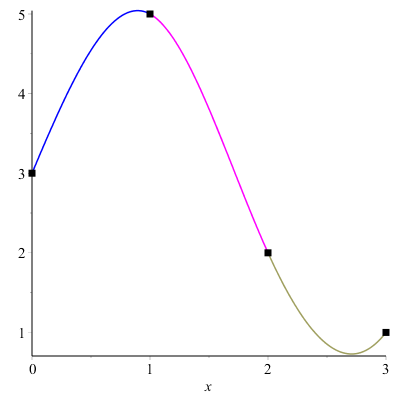
\includegraphics[scale=.5]{plots/problem4plot5.png}
\end{center}

%%%%%%%%%%%%%%%%%%%%%%%%%%%%%%%%%%%%%%%%%%%%%%%%%%%%


\section*{Problem 5}
\begin{enumerate}[i.)]
\item
\item
\item
\end{enumerate}




\section*{Problem 6}
\begin{enumerate}[i.)]
\item
\item
\item
\end{enumerate}





\section*{Problem 7}
\subsection*{$T_{10}(x)$}
%$$ \begin{array}{l l l}
%T_{10}(x) &= &512x^{10}-1280x^8+1120x^6-400x^4+50x^2-1\\
%T'_{10}(x) &= &5120x^9-10240x^7+6720x^5-1600x^3+100x \\
%T''_{10}(x) &= &46080x^8-71680x^6+33600x^4-4800x^2+100\\
%\int T_{10}(x) &= &\frac{512}{11}*x^{11}-\frac{1280}{9}x^9+160x^7-80x^5+\frac{50}{3}x^3-x
%\end{array}$$

\begin{tabular}{| c | c | c | c |}
\hline 
$n$ & $a_{T'_{10}}$ & $a_{T''_{10}}$ & $a_{\int T_{10}}$ \\
\hline \hline
0 & 0 & 500 & 0\\
1 & 20 & 0 & 0\\
2 & 0& 960 & 0\\
3 & 20& 0& 0\\
4 & 0 & 840& 0\\
5 & 20 & 0 & 0\\
6 & 0 & 640 & 0\\
7 & 20 & 0 & 0\\
8 & 0 & 360 & 0\\
9 & 20 & 0 & $\frac{1}{18}$\\
10 & 0 & 0 & 0\\
11 &  0& 0& $\frac{1}{22}$\\
\hline
\end{tabular}
\subsection*{$T_{15}(x)$}
%$$ \begin{array}{l l l}
%T_{15}(x) &= &16384x^{15}-61440x^{13}+92160x^{11}  -70400x^9+28800x^7-6048x^5+560x^3-15x\\
%T'_{15}(x) &= &245760x^{14}-798720x^{12}+1013760x^{10}-633600x^8+201600x^6-30240x^4+1680x^2-15\\
%T''_{15}(x) &= &3440640x^{13}-9584640x^{11}+10137600x^9-5068800x^7+1209600x^5-120960x^3+3360x \\
%\int T_{15}(x) &= &1024x^{16}-\frac{30720}{7}x^{14}+7680x^{12}-7040x^{10}+3600x^8-1008x^6+140x^4-\frac{15}{2}x^2
%\end{array}$$

\begin{tabular}{| c | c | c | c |}
\hline 
$n$ & $a_{T'_{15}}$ & $a_{T''_{15}}$ & $a_{\int T_{15}}$ \\
\hline \hline
0 & 15 & 0 & 0\\
1 & 0 & 3360 & 0\\
2 & 30& 0 & 0\\
3 & 0& 3240& 0\\
4 & 30 & 0& 0\\
5 & 0 & 3000 & 0\\
6 & 30 & 0 & 0\\
7 & 0 & 2640 & 0\\
8 & 30 & 0 & 0\\
9 & 0 & 2160 & 0\\
10 & 30 & 0 & 0\\
11 &  0& 1560 & 0\\
12 &  30& 0& 0\\
13 &  0& 840& 0\\
14 &  30& 0& $\frac{1}{28}$\\
15 &  0& 0& 0\\
16 &  0& 0& $\frac{1}{32}$\\
\hline
\end{tabular}
\subsection*{$T_{20}(x)$}
%$$ \begin{array}{l l l}
%T_{20}(x) &= &524288x^{20}-2621440x^{18}+5570560x^{16}-6553600x^{14}+4659200x^{12}-2050048x^{10}+ \\
%		& &549120x^8-84480x^6+6600x^4-200x^2+1\\
%T'_{20}(x) &= &10485760x^{19}-47185920x^{17}+89128960x^{15}-91750400x^{13}+55910400x^{11}-20500480x^9+ \\
%		& &4392960x^7-506880x^5+26400x^3-400x\\
%T''_{20}(x) &= &199229440x^{18}-802160640x^{16}+1336934400x^{14}-1192755200x^{12}+615014400x^{10} \\
%		& &- 184504320x^8+30750720x^6-2534400x^4+79200x^2-400 \\
%\int T_{20}(x) &= & \frac{524288}{21}x^{21}-\frac{2621440}{19}x^{19}+327680x^{17}-\frac{1310720}{3}x^{15}+358400x^{13}-186368x^{11} + \\
%			& & \frac{183040}{3}x^9-\frac{84480}{7}x^7+1320x^5-\frac{200}{3}x^3+x
%\end{array}$$

\begin{tabular}{| c | c | c | c |}
\hline 
$n$ & $a_{T'_{10}}$ & $a_{T''_{10}}$ & $a_{\int T_{10}}$ \\
\hline \hline
0 & 0 & 4000 & 0\\
1 & 40 & 0 & 0\\
2 & 0& 7920 & 0\\
3 & 40& 0& 0\\
4 & 0 & 7680& 0\\
5 & 40 & 0 & 0\\
6 & 0 & 7280 & 0\\
7 & 40 & 0 & 0\\
8 & 0 & 6720 & 0\\
9 & 40 & 0 & 0\\
10 & 0 & 6000 & 0\\
11 &  40& 0& 0\\
12 &  0& 5120& 0\\
13 &  40& 0& 0\\
14 &  0& 4080& 0\\
15 &  40& 0& 0\\
16 &  0& 2880& 0\\
17 &  40& 0& 0\\
18 &  0& 1520& 0\\
19 &  40& 0&  $\frac{1}{38}$\\
20 &  0& 0& 0\\
21 &  0& 0& $\frac{1}{42}$\\
\hline
\end{tabular}

\subsection*{Analysis}
The tables above list the coefficients $a_n$ of $T_n$ for all relevant $n$ for the first two derivatives and integral of each $T_n$. The patterns in the data can be explained by

$$T_n(x) = \frac{1}{2} \left( \frac{1}{n+1}T'_{n+1}(x) - \frac{1}{n-1}T'_{n-1}(x) \right)$$
which gives us 
$$\int T_n(x) = \frac{1}{2} \left(  \frac{1}{n+1}T_{n+1}(x) - \frac{1}{n-1}T_{n-1}(x) \right)$$
and
$$T_{n+1}(x) = 2xT_n(x) - T_{n-1}(x)$$
which gives
$$T'_n(x) = \frac{1}{1-x^2} \left( -nxT_n(x) + nT_{n-1}(x) \right)$$
which we can of course take the derivative of to obtain higher order derivatives of $T_n$.
\section*{Problem 8}
\subsection*{Lagrange Interpolation}
$L_8(x) = -10717.01390x^8 + 41523.43743x^7 - 66130.60764x^6 + 55973.20311x^5 - 27150.02639x^4 +7547.542702x^3 - 1112.916584x^2 + 66.38116670x + .302$\\
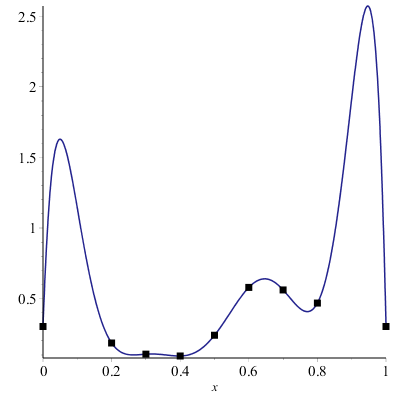
\includegraphics[scale=.5]{plots/problem7plot1.png}
\subsection*{Cubic Spline Interpolation}
$$
f(x) = \left\{
        \begin{array}{ll}
            .302 - .473x - 2.802x^3 &  x < 0.2 \\
            .12974+2.11093x-12.91926x^2+18.72996x^3 & x < 0.3 \\
 	.47410379-1.3326681x-1.44057x^2+5.975866x^3 & x < 0.4 \\
 	-2.430901+20.45487x-55.90942x^2+51.36657x^3 &  x < 0.5 \\
 	26.420189-152.651673x+290.3036659x^2-179.442153x^3 &  x < 0.6 \\
 	-37.6981566+167.940056x-244.015883x^2+117.40204x^3 & x < 0.7 \\
 	5.37168-16.644978x+19.67702x^2-8.1660098x^3 & x < 0.8 \\
 	1.257759-1.2177579x+.39299789x^2-.130999x^3 &  x \geq .8 \\
        \end{array}
    \right.
$$
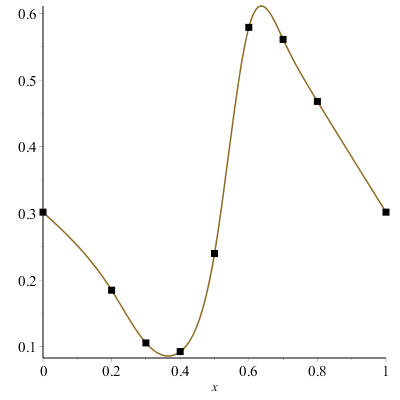
\includegraphics[scale=.5]{plots/problem7plot2.png}

\subsection*{Analysis}
The cubic spline interpolation produces a much more convincing interpolation between the data points - the Lagrange polynomial suffers from very erratic behavior
at the endpoints (similar to Runge's phenomenon), and indeed $f(.1) = 0.251906420711722$ is a much more consistent value with the data than $L_8(.1) = 1.14113749$. 



\end{document}
